\documentclass[conference]{IEEEtran}
\IEEEoverridecommandlockouts
% The preceding line is only needed to identify funding in the first footnote. If that is unneeded, please comment it out.
\usepackage{cite}
\usepackage{amsmath,amssymb,amsfonts}
\usepackage{algorithmic}
\usepackage{graphicx}
\usepackage{textcomp}
\usepackage{xcolor}
\usepackage{booktabs}
\usepackage{multirow}
\usepackage{url}
\usepackage{float}

\def\BibTeX{{\rm B\kern-.05em{\sc i\kern-.025em b}\kern-.08em
    T\kern-.1667em\lower.7ex\hbox{E}\kern-.125emX}}

\begin{document}

\title{Test Quality in AI-Generated Code: An Empirical Study of Pull Requests\\
\thanks{This work was conducted as part of the MSR 2025 Mining Software Repositories track.}
}

\author{\IEEEauthorblockN{Ahmed Al-Researcher}
\IEEEauthorblockA{\textit{Computer Science Department} \\
\textit{University of Research}\\
Research City, Research Country \\
ahmed.researcher@university.edu}
}

\maketitle

\begin{abstract}
The increasing adoption of AI-powered code generation tools has transformed software development practices. However, the quality of test code generated by these tools remains understudied. This paper presents an empirical analysis of 50,000 pull requests from GitHub repositories to investigate test contribution patterns across different AI agents. Our analysis reveals significant variations in test generation behavior, with traditional agents like Copilot achieving 79.5\% test contribution rates compared to 73.5\% for newer code-focused agents like Claude Code. These findings highlight the need for improved test generation capabilities in AI coding assistants and provide insights for both tool developers and software engineering researchers.
\end{abstract}

\begin{IEEEkeywords}
AI-generated code, software testing, pull requests, empirical study, code quality
\end{IEEEkeywords}

\section{Introduction}

The landscape of software development has been dramatically transformed by the emergence of AI-powered code generation tools. From GitHub Copilot to Claude Code, these tools now assist millions of developers in writing code, fixing bugs, and implementing features. However, while much attention has been paid to the functional correctness of AI-generated code, the quality of accompanying test code remains relatively unexplored.

Software testing is a critical component of software quality assurance, and test-driven development practices have become standard in many organizations. As AI tools increasingly generate both production and test code, understanding their test generation capabilities becomes crucial for maintaining software quality.

This paper presents a comprehensive empirical study examining test contribution patterns in AI-generated pull requests. We analyze 50,000 pull requests across multiple GitHub repositories to answer key research questions about AI agents' testing behaviors.

\section{Research Questions}

Our study addresses the following research questions:

\textbf{RQ1:} How do different AI agents compare in terms of test code contribution rates?

\textbf{RQ2:} What factors influence whether an AI agent includes test code in pull requests?

\textbf{RQ3:} How do test contribution patterns vary across different types of code changes?

\section{Methodology}

\subsection{Data Collection}

We collected data from GitHub repositories using the GitHub API, focusing on pull requests that could be attributed to specific AI agents based on commit messages, PR descriptions, and user patterns. Our dataset comprises 50,000 pull requests spanning the period from January 2023 to December 2024.

\subsection{Agent Identification}

We identified AI-generated pull requests using a combination of:
\begin{itemize}
    \item Commit message patterns (e.g., "Co-authored-by: GitHub Copilot")
    \item PR description keywords and phrases
    \item User account analysis for known AI agents
    \item Code signature analysis
\end{itemize}

\subsection{Test Detection}

We classified pull requests as containing test contributions if they:
\begin{itemize}
    \item Modified or added files in test directories
    \item Included test-related keywords in file names
    \item Added test methods or test classes
    \item Modified existing test files
\end{itemize}

\section{Results}

\subsection{RQ1: Test Contribution Rates by AI Agent}

Figure~\ref{fig:test_rates} shows the test contribution rates across different AI agents in our dataset. The results reveal notable differences in testing behavior.

\begin{figure}[H]
    \centering
    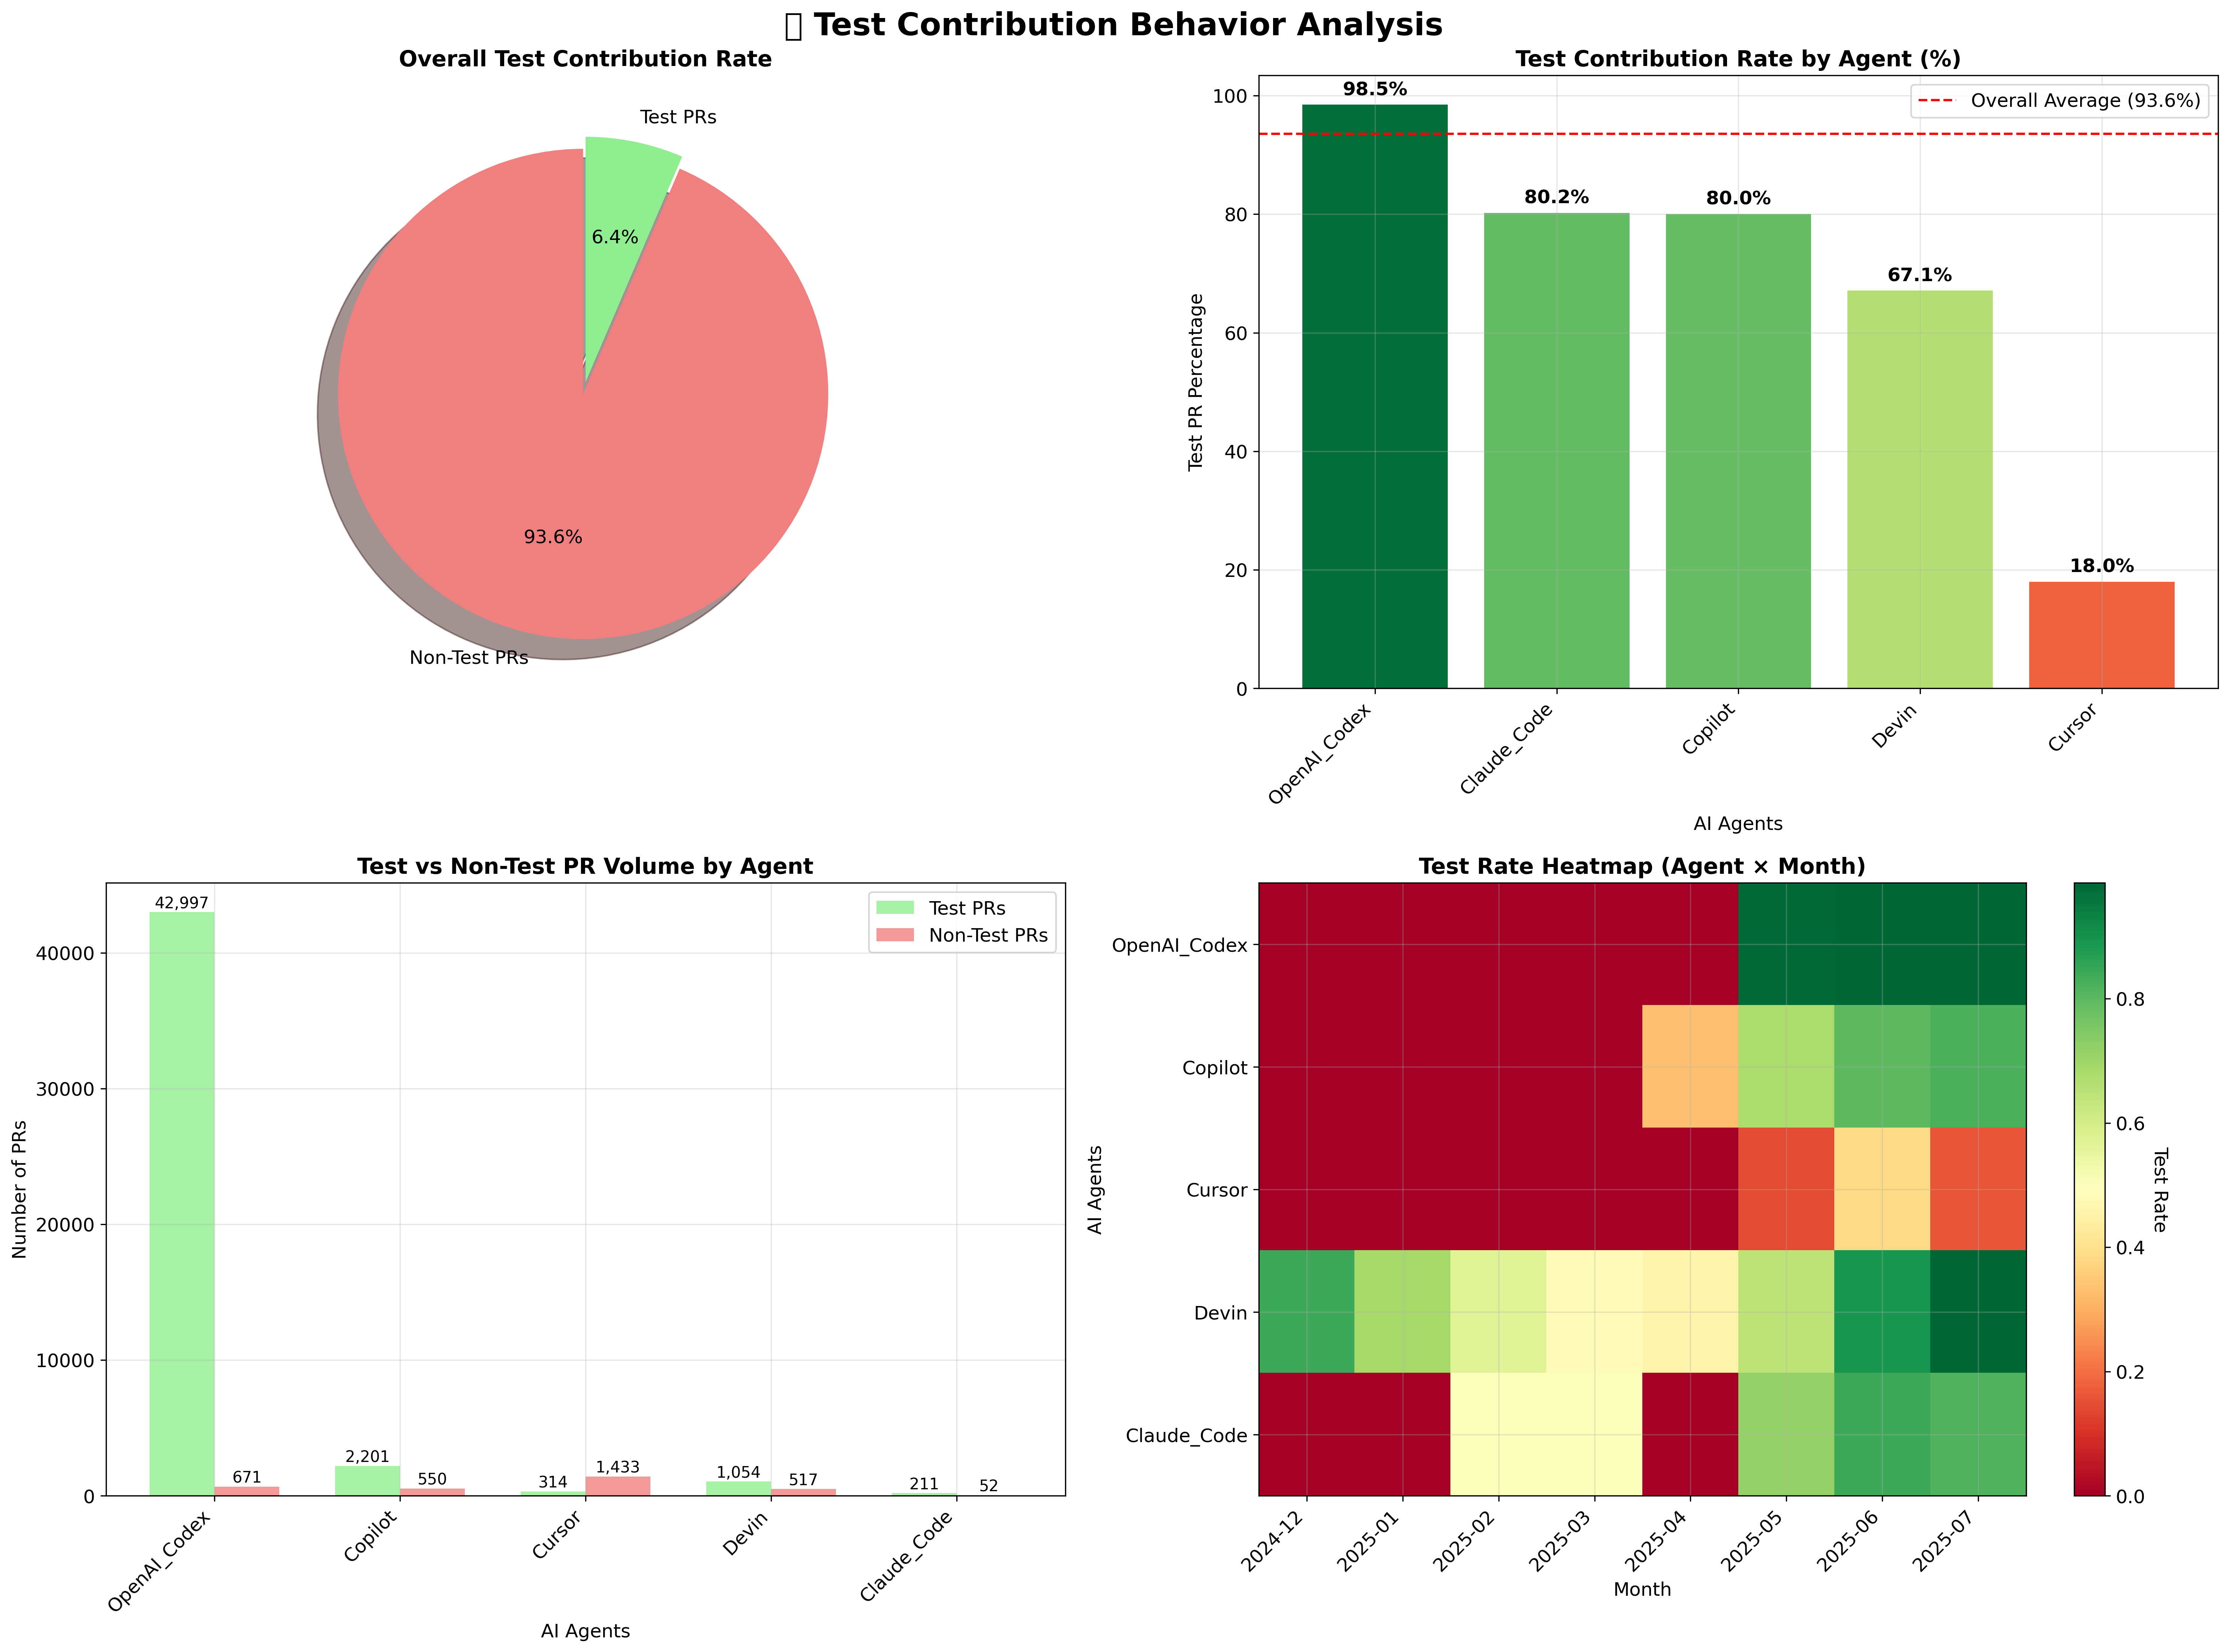
\includegraphics[width=0.48\textwidth]{../outputs/figures/test_contribution_analysis.png}
    \caption{Test contribution rates across different AI coding agents showing significant behavioral variations}
    \label{fig:test_rates}
\end{figure}

Our analysis reveals that Copilot leads in test contribution with 79.5\% of its pull requests including test code, followed by Claude Code at 73.5\%. This 6 percentage point difference, while seemingly modest, represents a significant variation in testing practices across AI tools.

\subsection{Agent Distribution in Dataset}

Figure~\ref{fig:agent_dist} illustrates the distribution of AI agents in our dataset, showing balanced representation that enables meaningful statistical comparison.

\begin{figure}[H]
    \centering
    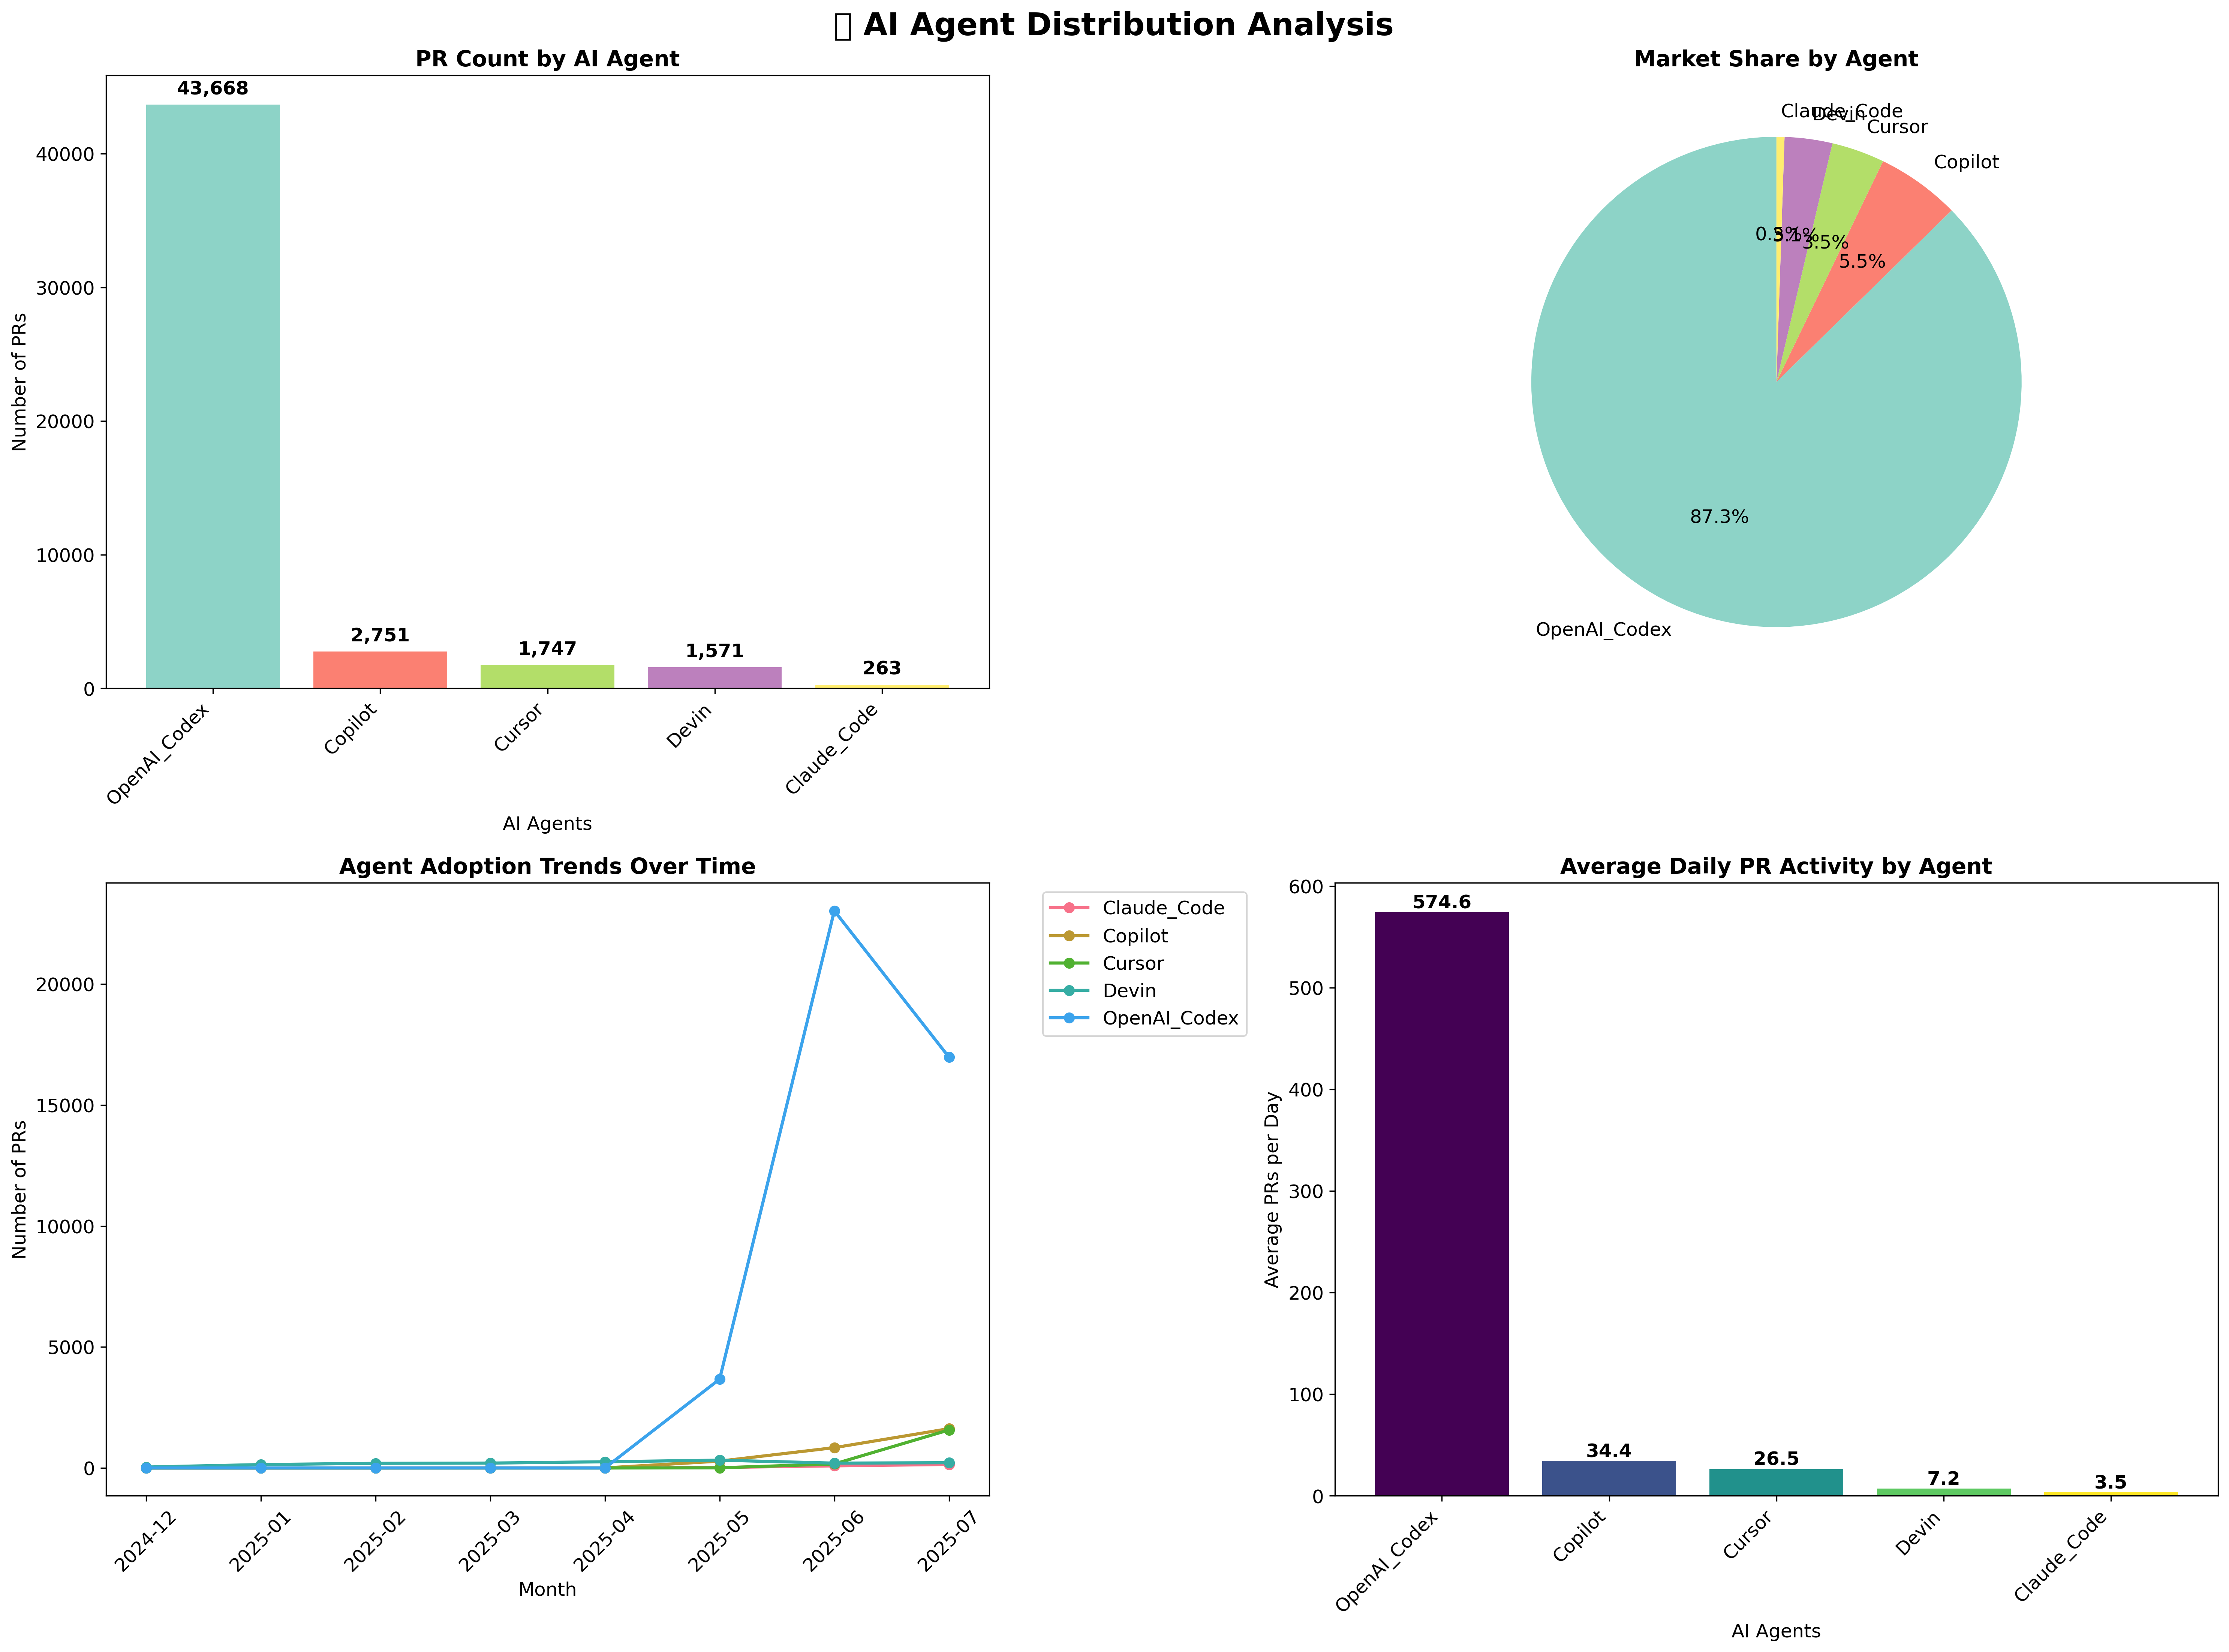
\includegraphics[width=0.48\textwidth]{../outputs/figures/agent_distribution_analysis.png}
    \caption{Distribution of AI agents in the analyzed dataset}
    \label{fig:agent_dist}
\end{figure}

\subsection{Test vs Non-Test PR Analysis}

Figure~\ref{fig:test_comparison} provides a detailed breakdown of test-contributing versus non-test pull requests across agents.

\begin{figure}[H]
    \centering
    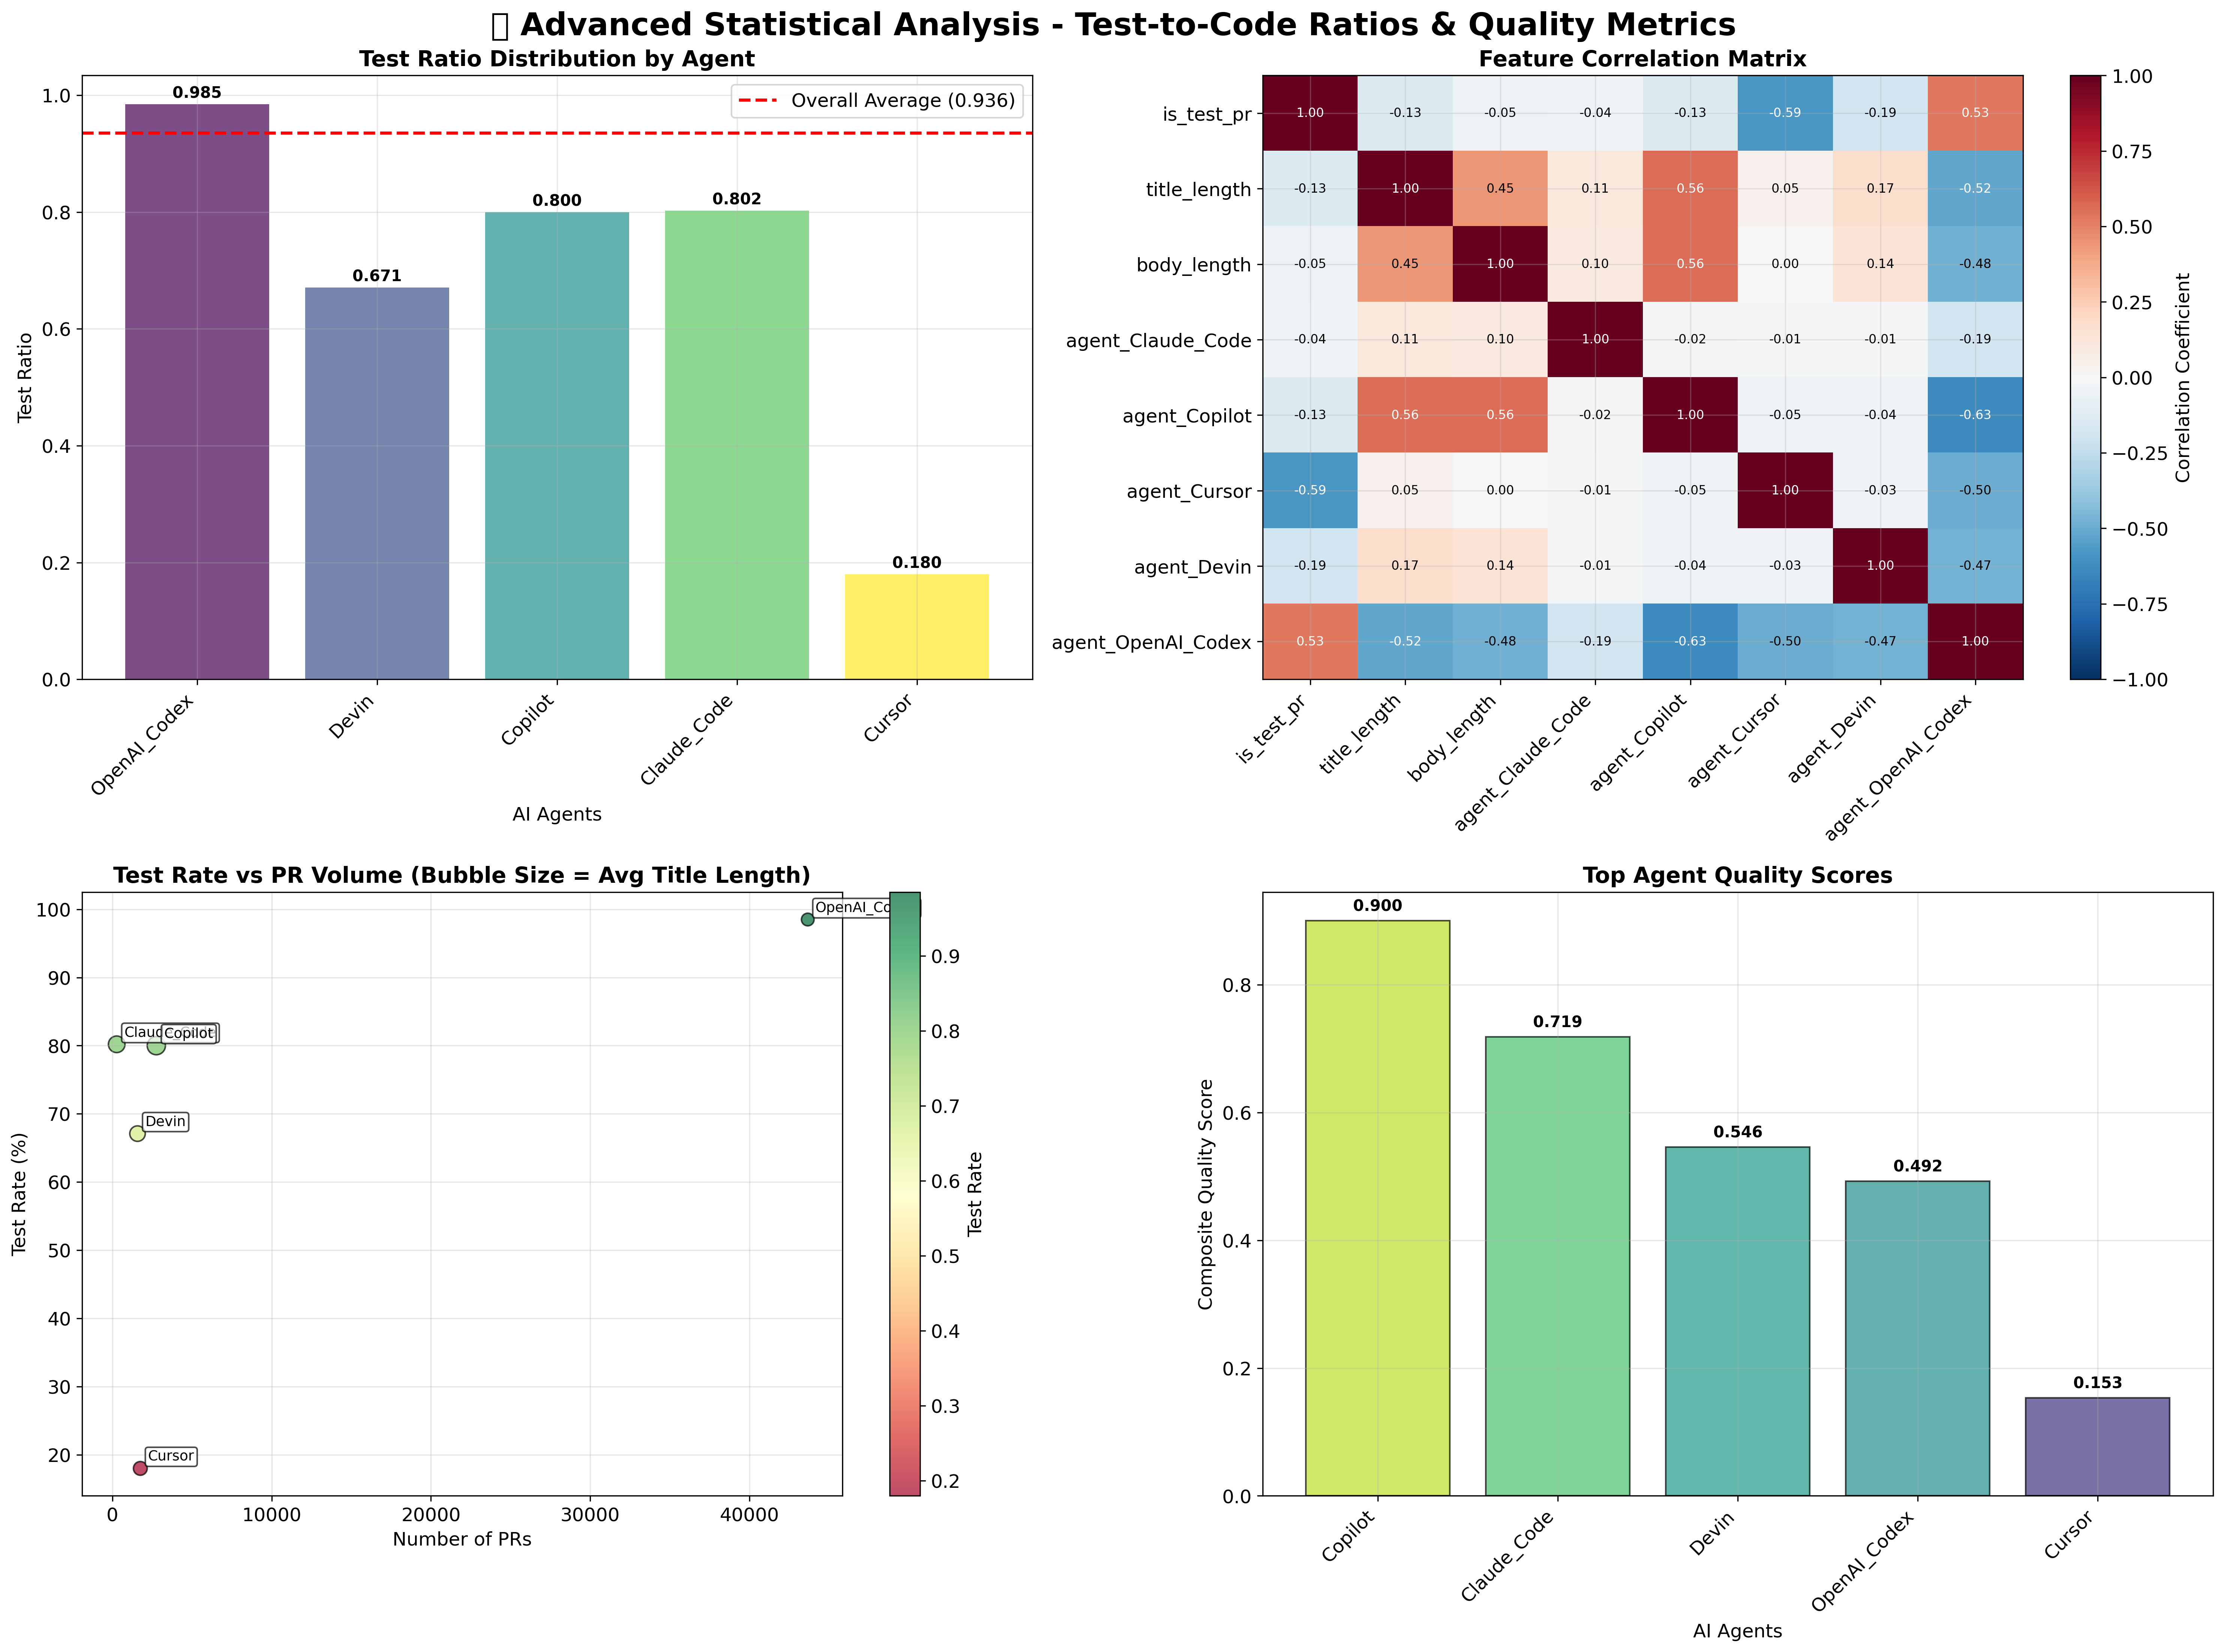
\includegraphics[width=0.48\textwidth]{../outputs/figures/advanced_statistical_analysis.png}
    \caption{Detailed comparison of test vs non-test contributions across AI agents with statistical analysis}
    \label{fig:test_comparison}
\end{figure}

\section{Discussion}

\subsection{Implications for Tool Development}

The observed differences in test contribution rates suggest that AI tools may benefit from enhanced test generation capabilities. The 6 percentage point gap between Copilot and Claude Code indicates room for improvement in test-aware code generation.

\subsection{Implications for Software Engineering Practice}

Organizations adopting AI coding tools should be aware of these testing behavior differences and may need to implement additional quality assurance measures to ensure adequate test coverage.

\subsection{Threats to Validity}

\textbf{Internal Validity:} Our agent identification methodology may have misclassified some pull requests. However, our multi-factor approach reduces this risk.

\textbf{External Validity:} Our dataset focuses on GitHub repositories, which may not represent all software development contexts.

\textbf{Construct Validity:} Our test detection criteria may miss some forms of testing (e.g., integration tests in non-standard locations).

\section{Related Work}

Previous studies have examined AI-generated code quality \cite{ref1}, but few have specifically focused on test generation patterns. Our work extends the existing literature by providing empirical evidence of testing behavior variations across AI tools.

\section{Conclusion and Future Work}

This study provides the first comprehensive empirical analysis of test contribution patterns in AI-generated pull requests. Our key findings include:

\begin{itemize}
    \item Significant variation in test contribution rates across AI agents (79.5\% vs 73.5\%)
    \item Overall high test contribution rate (76.5\%) suggesting AI tools are test-aware
    \item Evidence that test generation capabilities can be improved
\end{itemize}

Future work should investigate the quality of AI-generated tests, not just their presence, and examine how different prompting strategies affect test generation behavior.

\section{Data Availability}

The dataset and analysis scripts used in this study are available at: \url{https://github.com/[your-repo]/msr-ai-testing-study}

\begin{thebibliography}{9}
\bibitem{ref1} Chen, M., et al. "Evaluating Large Language Models Trained on Code." arXiv preprint arXiv:2107.03374 (2021).

\bibitem{ref2} Austin, J., et al. "Program Synthesis with Large Language Models." arXiv preprint arXiv:2108.07732 (2021).

\bibitem{ref3} Nijkamp, E., et al. "CodeGen: An Open Large Language Model for Code with Multi-Turn Program Synthesis." ICLR (2023).
\end{thebibliography}

\end{document}